\chapter{Automaty komórkowe}

\section{Zagadnienie automatów}

\noindent Ciekawym zagadnieniem dotyczącym dzisiejszej informatyki jest symulacja  różnego rodzaju zjawisk, wydarzeń i populacji. Interesującą właściwością symulowanych modelów jest złożoność zachowań przy nakreśleniu prostych reguł działania. Na myśl nasuwa się pytanie: jakie zachowania będą przejawiały systemy zamodelowane bardziej wyrafinowanymi zasadami. Ograniczenia systemu w połączeniu z modelami matematycznymi oraz mocą obliczeniową komputerów mogą dać ciekawe rezultaty, których moglibyśmy nie przewidzieć. Utworzenie odpowiedniego modelu i wybranie odpowiednich warunków początkowych, pozwala nam też sprawdzić jak zachowa się dany system.
\noindent W celu zrealizowania podanego systemu jako program komputerowy na pomoc przychodzą nam automaty komórkowe. Dzięki prostocie zasad ich działania w bardzo krótkim czasie jesteśmy w stanie stworzyć prosty mechanizm, który będzie symulował rozwój populacji zwierząt. Stopniowo wprowadzając zasady działania populacji, od najprostszych jakimi jest poruszanie się i zdobywanie pokarmów, po te bardziej skompilowane jakimi jest rozmnażanie, uciekanie przed drapieżnikami czy polowanie na inne zwierzęta. Naszą uwagę przykuł fakt jak prosty jednowymiarowy automat komórkowy o prostych zasadach funkcjonowania może, przy niewiele różniących się od siebie regułach, dać zupełnie inny obraz wynikowy. Należy też zauważyć, że najwięcej funkcjonalności automatów komórkowych możemy znaleźć analizują właśnie jednowymiarowe  automaty. Tutaj definiujemy komórke oraz jej sąsiednie komórki, które znajdują się w pewnej odległości od niej. Dzięki temu jesteśmy za pomocą funkcji przejścia wyznaczyć następny stan danej komórki. 
\noindent Zaczniemy od tablicy jednowymiarowej i oznaczymy sobie dwa stany: 1 jako komórkę żywą, 0 jako komórkę  martwą, a jako sąsiadów przyjmiemy tylko te komórki,które znajdują się bezpośrednio przy niej. Ustalimy też, że następny stan będzie zależał bezpośrednio od stanu samej komórki oraz stanu sąsiadów. Wybierzemy też przejścia takie jak na tablicy.

\begin{table}[h!]
\centering
\begin{tabular}{ |c|c|c|c|c|c|c|c| } 
	\hline
	111 & 110 & 101 & 100 & 011 & 010 & 001 & 000\\
	0 & 0 & 1 & 0 & 0 & 1 & 1 & 0 \\
	\hline
\end{tabular}
\label{table:1}
\end{table}
\clearpage

\begin{figure}[ht]
	\centering
	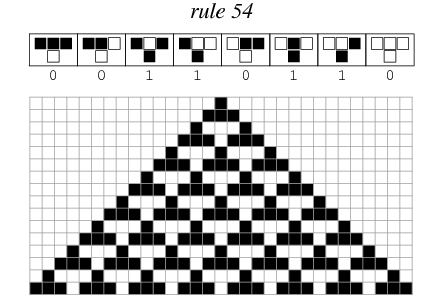
\includegraphics[width=0.8\textwidth]{img/triangle}
	\caption{rezultat wykonania operacji wedle tablicy powyżej}
\end{figure}

\section{Implementacja automatu}

\noindent Modelowanie populacji drapieżnik-ofiara za pomocą automatów komórkowych jest złożoną operacją. Każda komórka to zbiór stanów poszczególnych osobników. Każdy następny stan bazuje na poprzednim oraz na stanach sąsiadów.

\noindent Autorzy książki "A predator-prey model based on fully parallel cellular automata" przeprowadzi symulację na podstawie populacji wilków i owiec. Udało im się znaleźć trzy możliwe stany, do których będzie dochodził system. Są nimi:

\begin{itemize}
	\item współistnienie obu gatunków,
	\item rozwijanie się populacji ofiar,
	\item wyginięcie obu gatunków
\end{itemize}

\noindent Te stany zależały od ilości pożywania dla ofiar, czasu po jakim zwierzęta były wstanie się rozmnażać oraz sposobem opiekowania się na młodymi. Największym problemem z jakim spotkali się twórcy było to, że drapieżnik podczas polowania mógł zabić klika ofiar. Sposobem na poradzenia sobie  z tego typu zjawiskiem było wprowadzenie specjalnego sposobu doboru sąsiedztwa, które nie występowała w innych  automatach, a pozwala blokować możliwość zabicia wszystkich ofiar.  Dodatkowo dyskutowali też jaki wpływ na rozwoje populacji będą mieć takie czynniki jak zagęszczenie oraz mutacje poszczególnych gatunków. Zastanawiali się też jakie wtedy stany może osiągnąć taki automat.